%!TEX root = ../main.tex



\section{Εισαγωγή}

\lettrine[findent=2pt]{\fbox{\textbf{Σ}}}{τα} προηγούμενα κεφάλαια έγινε ανάλυση των κλασικών μεθόδων ρύθμισης ενός PID ελεγκτή και παρουσιάστηκαν οι τρόποι με τους οποίους ο κάθε όρος του ελεγκτή επηρεάζει την απόκριση του τελικού συστήματος. Σε αυτό το κεφάλαιο παρουσιάζεται ο αυτο-ρυθμιζόμενος PID ελεγκτής που αναπτύχθηκε στα πλαίσια της διπλωματικής μου εργασίας. Αρχικά, γίνεται αναφορά στη θεωρία που αφορά την αυτόματη ρύθμιση του ελεγκτή. Στη συνέχεια, παραθέτονται λεπτομέρειες και επεξηγήσεις για τη δομή του προγράμματος που φτιάχτηκε σε LabVIEW.  Τέλος, γίνεται σχολιασμός των πειραματικών αποτελεσμάτων που προκύπτουν από την προσομοίωση των διάφορων συστημάτων ελέγχου στον υπολογιστή.

\section{Θεωρία}

\lettrine[findent=2pt]{\fbox{\textbf{Μ}}}{ε} τον όρο \emph{``αυτο-ρυθμιζόμενος" PID ελεγκτής} ή \emph{αυτόματη ρύθμιση του PID ελεγκτή} εννοούμε μία μέθοδο στην οποία τα κέρδη του ελεγκτή ρυθμίζονται αυτόματα μετά από απαίτηση του χρήστη. Συνήθως, ο χρήστης θα πατήσει ένα κουμπί ή θα στείλει μια εντολή στον ελεγκτή. Μια αυτόματη ρύθμιση του ελεγκτή περιλαμβάνει τα εξής τρία βήματα:

\begin{itemize}
	\item Δημιουργία μιας διαταραχής του συστήματος.
	\item Εκτίμηση της απόκρισης που προκαλεί η διαταραχή.
	\item Υπολογισμός των παραμέτρων του ελεγκτή.
\end{itemize}
Αυτά αποτελούν και τα βήματα που εκτελεί και ένας έμπειρος ελεγκτής όταν κάνει χειροκίνητη ρύθμιση του ελεγκτή. Το σύστημα πρέπει να διαταραχθεί με κάποιον τρόπο έτσι ώστε να εκτιμηθούν οι δυναμικές που το διέπουν. Αυτό μπορεί να γίνει με πολλούς τρόπους όπως, για παράδειγμα, εισάγοντας ημιτονοειδή σήματα, παλμούς ή βηματικές αλλαγές στην είσοδο του συστήματος.

\subsection{Relay Method}
Η μέθοδος που χρησιμοποιήθηκε σε αυτή την εργασία είναι αυτή που στη βιβλιογραφία αναφέρεται ως \emph{``Relay Method"} (δεν υπάρχει ακριβής μετάφραση στα ελληνικά) \cite{astrom}, \cite{vandoren}. Η μέθοδος αυτή βασίζεται, όπως και οι μέθοδοι \emph{Ziegler-Nichols} και \emph{Tyreus-Luyben}, στην απόκριση συχνότητας του συστήματος.

Στην πραγματικότητα, η μέθοδος \emph{Ziegler-Nichols}, όπου το κέρδος που φέρνει το σύστημα στην οριακή ευστάθεια βρίσκεται πειραματικά, είναι μια μορφή αναγνώρισης μοντέλου. Όλες οι τεχνικές ρύθμισης στην πραγματικότητα περιέχουν κομμάτια αναγνώρισης μοντέλου,
αλλά οι πιο δημοφιλείς απλά βελτιώνουν και αποκρύπτουν αυτά τα κομμάτια καλύτερα. Στην ουσία, όλη η διαδικασία ρύθμισης χρησιμοποιώντας τη μέθοδο Ziegler-Nichols γίνεται για να βρεθεί το κέρδος στο οποίο το σύστημα έχει μισό κύκλο καθυστέρηση όταν λειτουργεί σε ανατροφοδότηση. Αυτό είναι που αναφέρθηκε στην Ενότητα \ref{subsec:Ziegle-Nichols Method} ως απόλυτο κέρδος $K_u$ και σχετίζεται με το σημείο όπου η καμπύλη Nyquist του συστήματος κόβει πρώτα τον πραγματικό άξονα, όπως φαίνεται στο Σχήμα \ref{fig:nyquist}.

\begin{figure}[h]
  \centering
  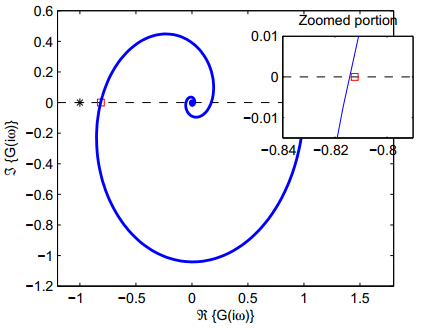
\includegraphics[width=\textwidth]{nyquist}
  \caption{Διάγραμμα Nyquist ενός ανοιχτού σταθερού συστήματος με κάποια καθυστέρηση (deadtime)}
  \label{fig:nyquist}
\end{figure}

Το πρόβλημα με τη μέθοδο αυτή είναι ότι για να βρεθεί το απόλυτο κέρδος, το σύστημα θα πρέπει να φτάσει στα όρια του, με ό,τι αρνητικές συνέπειες μπορεί να επιφέρει αυτό, τόσο στη λειτουργία του όσο και στην κατασκευή του. Η μέθοδος ``Relay" που περιγράφεται εδώ καταφέρνει να βρίσκει πειραματικά τόσο το απόλυτο κέρδος όσο και την απόλυτη συχνότητα του συστήματος. Τα βήματα που ακολουθούνται για την εφαρμογή της μεθόδου είναι τα ακόλουθα:
\begin{enumerate}

\item Προσωρινά, ο ελεγκτής δίνει τη θέση του σε μία μη γραμμική συνάρτηση (στην ουσία είναι on-off	έλεγχος) (Σχήμα \ref{fig:relay}) η οποία εναλλάσσει την είσοδο του συστήματος μεταξύ δύο διακριτών τιμών. Κάθε φορά που η τιμή του σφάλματος $e(t)$ (δηλαδή $setpoint - output$) είναι μεγαλύτερη από το μηδέν η έξοδος του relay στοιχείου είναι $d$. Κάθε φορά που η τιμή του σφάλματος $e(t)$ είναι μικρότερη από το μηδέν η έξοδος του relay στοιχείου είναι $-d$.

\item Αποφεύγοντας την εις βάθος μαθηματική ανάλυση \cite{astrom}, η αντικατάσταση του ελεγκτή με ένα relay στοιχείο, εξαναγκάζει το σύστημα να εκτελεί ταλαντώσεις σταθερού πλάτους και συχνότητας (Σχήμα \ref{fig:relay2}). Η συχνότητα αυτή είναι σχεδόν ίδια με την απόλυτη συχνότητα του συστήματος, ενώ το απόλυτο κέρδος είναι αντιστρόφως ανάλογο του πλάτους της παρατηρούμενης ταλάντωσης.

\item Περιμένουμε η απόκριση του συστήματος να σταθεροποιηθεί σε αμείωτες ταλαντώσεις σταθερής συχνότητας και καταγράφουμε το πλάτος $\alpha$ και την περίοδο $T$.
 
\item Η παρατηρούμενη περίοδος είναι η απόλυτη περίοδος, δηλαδή $T_u=T$, ενώ το απόλυτο κέρδος συνδέεται με το πλάτος $\alpha$ με τη σχέση,
\begin{equation}
K_u = \frac{4d}{\pi\alpha}
\end{equation}

\item Έχοντας υπολογίσει το απόλυτο κέρδος και την απόλυτη περίοδο, μπορούν να οριστούν τα κέρδη του PID ελεγκτή με βάση τους Πίνακες \ref{table:zn_method} και \ref{table:tl_method} των μεθόδων Ziegler-Nichols και Tyreus-Luyben αντίστοιχα.

\end{enumerate}

\begin{figure}[h]
  \centering
  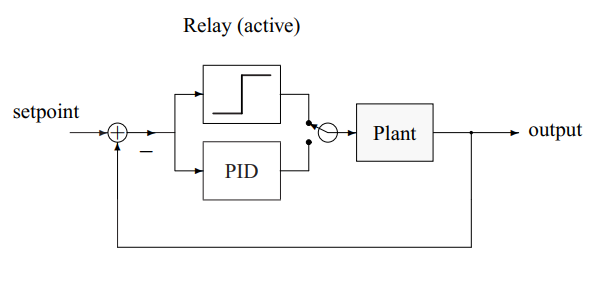
\includegraphics[width=\textwidth]{relay}
  \caption{Δομικό διάγραμμα συστήματος με relay στοιχείο}
  \label{fig:relay}
\end{figure}



Η διαδικασία της αντικατάστασης του PID ελεγκτή με το relay στοιχείο, η μέτρηση του πλάτους και της περιόδου των ταλαντώσεων και ο υπολογισμός των κερδών του ελεγκτή μπορεί να αυτοματοποιηθεί αξιόπιστα. Αυτή η μέθοδος χρησιμοποιείται και σε εμπορικά διαθέσιμους PID ελεγκτές. Σημαντικό πλεονέκτημα της μεθόδου αυτής σε σχέση με τη μέθοδο Ziegler-Nichols είναι ότι το σύστημα δεν χρειάζεται να διεγείρεται στα όρια του. Επειδή το πλάτος των ταλαντώσεων $\alpha$ είναι ανάλογο του πλάτους $d$ του relay, μπορούμε να ορίσουμε το πλάτος $\alpha$ έτσι ώστε οι ταλαντώσεις να μην είναι υπερβολικά μεγάλες και, κατά συνέπεια, επικίνδυνες για το σύστημα ή τον εξοπλισμό.

\begin{figure}[H]
  \centering
  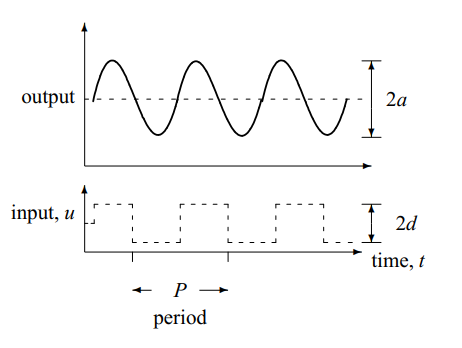
\includegraphics[width=\textwidth]{relay2}
  \caption{Ταλαντώσεις ενός συστήματος υπό συνθήκες ανατροφοδότησης μέσω relay στοιχείου αντί για ελεγκτή.}
  \label{fig:relay2}
\end{figure}

\section{Το Πρόγραμμα}

\lettrine[findent=2pt]{\fbox{\textbf{Σ}}}{την} ενότητα αυτή θα παρουσιαστεί το πρόγραμμα σε LabVIEW που υλοποιεί τον αυτο-ρυθμιζόμενο PID ελεγκτή. Για την καλύτερη οργάνωση του προγράμματος, το κυρίως VI αποτελείται από επί μέρους subVIs που το καθένα επιτελεί διαφορετική λειτουργία του προγράμματος. Σε κάθε υποενότητα λοιπόν θα παρουσιάζεται ένα από αυτά τα subVIs και θα αναλύεται η δομή του καθώς και η λειτουργία που επιτελεί.

\subsection{Το Front Panel και το Block Diagram}





















